\section{Sequence Prediction}
As machine learning is a very broad field covering tons of different applications, use cases and is based on differing assumptions it is crucial to first analyze what kind of problem is supposed to be tackled by applying machine learning techniques to it. Without a fond and thorough understanding of the domain and the available data it's almost impossible to get a useful result and conclusion from doing experiment. Just as it is a lot harder for a normal human being to deduce useful information and to learn something given some random, unstructured, unprepared, redundant or even wrong data it is also not possible (at least not yet) for a computer (i.e. a machine learning algorithm) to simply make sense of a heap of data. Data needs to be analyzed, prepared, structured and combined before being fed to the algorithm in order for it to fully unveil its usefulness. If we do not properly prepare the data we are almost certain to run into indescribable issues or results later on in the process.

Many machine learning algorithms are created for independent, identically distributed data. They work under the assumptions that two data points should not correlate and have no explicit influence on each other. In our thesis this is not the case. We explicitly combine data from different data points (such as what was the last station before this one). Therefore we have modeled our problem as a sequence prediction, or sequence learning problem. Why we used sequence description is described in section~\ref{subsec:task_description}. 

Sequence prediction deals with sequential data. A machine learning algorithm that allows for sequential data should not make the assumption that the data points are independent, should account for distortion and should also use contextual information, whenever available. Popular use cases for algorithms using sequence prediction are time-series predictions (e.g. weather forecasting, stock market predictions, geographical tracking predictions) and sequence labeling (e.g. speech recognition, handwriting recognition, gesture recognition). There are different types of algorithms that fall under this technique, such as different supervised learning classifiers (e.g. Decision Trees, Probabilistic Algorithms, Support Vector Machines, Neural Networks). In our experiments we have included several different algorithms out of the field of sequence prediction.

\subsection{Task Description}
\label{subsec:task_description}
We model our problem as a sequence prediction problem due to the fact that we have to work with heavily dependent individual data points. Due to the way our data is structured we need to assume that different data points rely on each other. As will be explained in more detail in section~\ref{subsec:data_set} we gather a number of values for every data point. Among these values are the current station (mapped as an id), the anonymized user id and a timestamp. While preparing our data we enhance the data points with references to the previous and the next station.


\subsection{Proposed Solutions}
\label{subsec:proposed_solution}
We used multiple different techniques to solve our task and to use in the final evaluation. Decision Trees and Random Forests, a Naive Bayes algorithm as well as Hidden Markov Models (which fall under the Neural Networks category). The theoretical foundation of these algorithms are described here in further detail. The practical way in which we used them are described in Section~\ref{subsec:machine_learning_results}

\subsubsection{WEKA}

\subsubsection{Decision Trees}
Decision tree learning in the context of data mining is a technique using a decision tree as a predictive model to map observation about input data to come to a conclusion about the data's target value. A tree model that accepts a finite set of values is called a "classification tree", in case continuous values are allowed the decision tree is called "regression tree". A decision tree doesn't explicitly represent a decision, however the resulting classification tree can be used as an input for decision making. 

In a decision tree model, a leaf represents a class label and a branch represents a conjunction of features leading to the class labels. As can be seen in the example in Figure \ref{fig:image-decision-tree} the interior nodes correspond to the input values, the edges are the value domain and the leafs represent the values of the target variable. With such a modeled decision tree we can easily either visually or computationally evaluate new input data and derive the target values.

\begin{figure}[!ht]
	\centering
		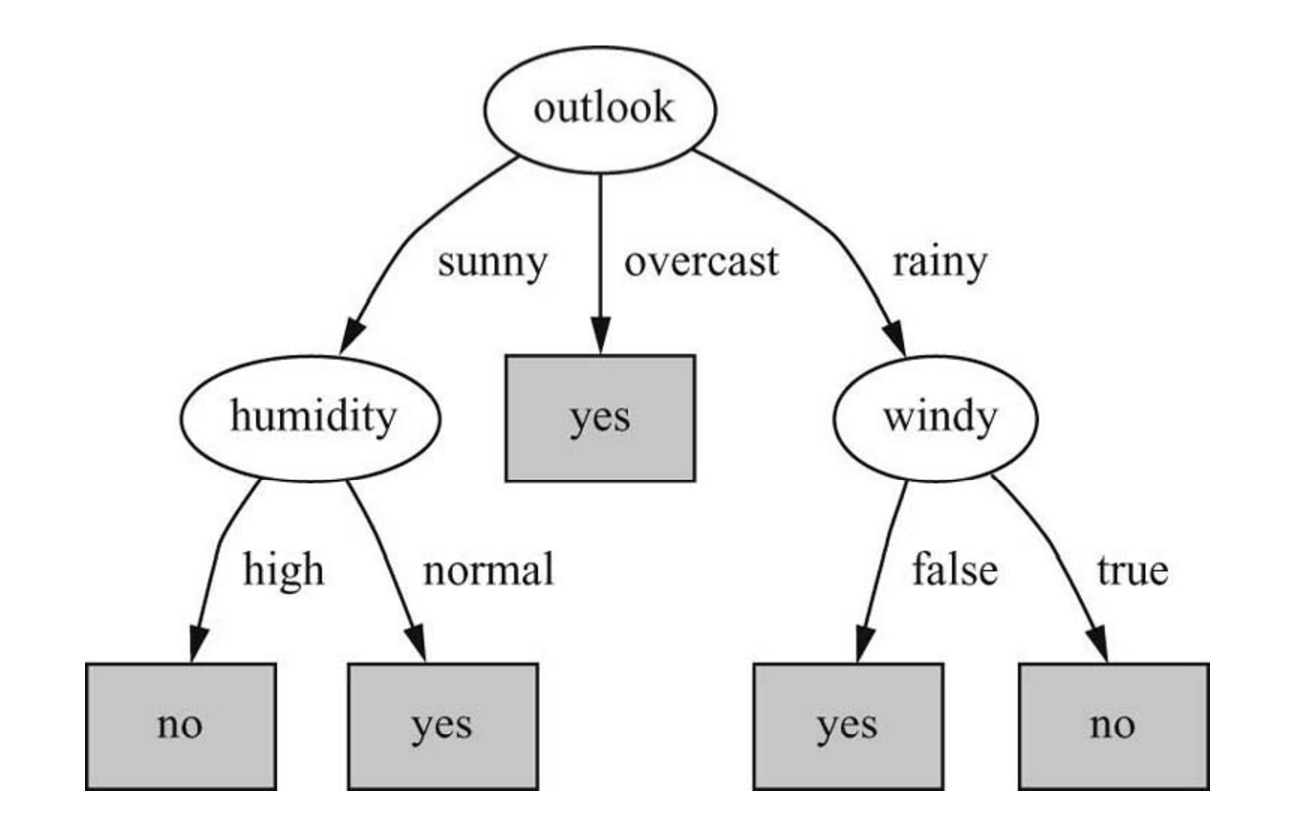
\includegraphics[width=1.0\textwidth]{images/decision-tree}
	\caption{An example of a decision tree}
	\label{fig:image-decision-tree}
\end{figure}

A tree can be trained or learned by splitting the source data set into subsets based on testing the attribute values. In order to get the full model of the decision tree, this process has to be repeated until a subset at a node has only one value or until splitting no longer adds value to the predictions. This process is called recursive partitioning and it is the most common strategy to train decision trees.


---- IS THIS FINALLY LEGAL? ------
\bibliography{https://en.wikipedia.org/wiki/Decision_tree_learning}

\subsubsection{Naive Bayes}
Here goes the theoretical description of Naive Bayes

\subsubsection{HMM / Neural Networks / Multilayer Perceptron}
Here goes the theoretical description of Hidden Markov Models and Neural Networks